\documentclass[10pt]{article}

\usepackage{amssymb,amsmath}
\usepackage{graphicx}
\usepackage{natbib}

%% THE USEPACKAGES NECESSARY FOR THIS EXAMPLE
%% NOTE THAT genetics_manu_style MUST BE CALLED AFTER mychicago
% \usepackage{graphicx}
% \usepackage{endfloat}
% \usepackage{amsfonts}
% \usepackage{subfigure}
% \usepackage{genetics_manu_style}

% \usepackage{siunitx}
% \sisetup{output-exponent-marker=\ensuremath{\mathrm{E}}}

% % Add hyperlinks
% %\usepackage{hyperref}

% % amsmath package, useful for mathematical formulas
% \usepackage{amsmath}
% % amssymb package, useful for mathematical symbols
% \usepackage{amssymb}

% % graphicx package, useful for including eps and pdf graphics
% % include graphics with the command \includegraphics
% \usepackage{graphicx}

% % cite package, to clean up citations in the main text. Do not remove.
% %\usepackage{cite}
% \usepackage{natbib}
% \bibpunct{(}{)}{;}{author-year}{}{,} 

% \usepackage{color}


% % Use doublespacing - comment out for single spacing
% \usepackage{setspace}

% % For splitting/combining figures.
% \usepackage{subfigure}

% % Use doublespacing - comment out for single spacing
% %\usepackage{setspace} 
% %\doublespacing

% % Split table cells
% %\usepackage{slashbox}

% % Table with curly braces
% \usepackage{multirow,bigdelim}

% % Underline 
% \usepackage[normalem]{ulem}


\newcommand{\St}{\mathcal{S}}
\newcommand{\It}{\mathcal{I}}
\newcommand{\Rt}{\mathcal{R}}
\newcommand{\traj}{\mathcal{V}}

\newcommand{\tree}{\mathcal{T}}

\newcommand{\comment}[1]{{\color{red} (#1)}}

\newcommand{\stochCoalSIR}{stochastic coalescent SIR}
\newcommand{\deterCoalSIR}{deterministic coalescent SIR}

\newcommand{\StochCoalSIR}{Stoch. Coal. SIR}
\newcommand{\DeterCoalSIR}{Deter. Coal. SIR}


\newcommand{\stochSIR}{stochastic SIR}
\newcommand{\StochSIR}{Stochastic SIR}
\newcommand{\BDSIR}{BDSIR}

\title{Supporting material for ``Bayesian Coalescent Epidemic Inference:  Comparison of Stochastic and Deterministic SIR Population Dynamics''}
\date{}

%% BEGIN DOC
\begin{document}

\maketitle{}

% \begin{center}
% \LARGE{Epidemic Parameter Inference with Coalescent SIR} \\
% \Large{Supplementary Material}
% \end{center}

\section{Sampling from the prior}

In order to assess the correctness of our implementation of the
deterministic coalescent SIR and stochastic coalescent SIR models, for
each model we used the MCMC algorithm to sample trees from the
corresponding distribution $f(\tree|\eta)$, and compared these samples
with coalescent trees simulated directly under the model.

The chosen $\eta$ included $\beta=7.5\times 10^{-4}$, $\gamma=0.3$,
$S_0=999$ and $z_0=30$. The comparisons were performed for trees
generated from 20 leaves, sampled at integer times 0 through 19,
inclusive.

For the deterministic coalescent SIR model, the direct simulation
involved numerically solving the Eqs.~(1)--(3) in the main text for
$t\in[0,30]$ and using this solution in combination with Eq.~(10)
in the main text to determine the instantaneous coalescent rate
$\lambda(\tau)$. This rate was used to simulate each of the coalescent
trees in the usual fashion for heterochronous leaf times.  In the case
that the MRCA was not reached before the origin time of the epidemic,
the tree was discarded and the simulation repeated.

The direct simulation proceeded in a similar way for the stochastic
coalescent SIR model, the major difference being that the
stochasticity of this model required each coalescent tree to be
simulated under a distinct realization of the stochastic trajectory.

Comparisons between the direct simulation and MCMC results are shown
in Figures \ref{fig:detCoalValidation} and
\ref{fig:stochCoalValidation} for three different summary
statistics and show very close agreement.

\section{Measuring inference accuracy and precision}
Following \cite{Kuhnert:2014}, the precision and accuracy of these methods were measured by 
relative error, bias, and highest posterior density (HPD) intervals using as an estimate the posterior 
median value of the parameter value $\overset{\wedge}{\eta}$, compared with the true parameter 
$\bar{\eta} = (R_{0}, \gamma, S_{0}, z_{0})$.  Error and bias are gauged by calculating the 
median value over medians from all 100 trials, such that:

$$\text{relative error} = \frac{\sum\nolimits_{\tau = 1}^{100}\frac{|\overset{\wedge}{\eta} - 
\bar{\eta}|}{\bar{\eta}}}{100} $$

\begin{center}
and
\end{center}
$$\text{relative bias} = \frac{\sum\nolimits_{\tau = 1}^{100}\frac{\overset{\wedge}{\eta} - 
\bar{\eta}}{\bar{\eta}}}{100} . $$

\vspace{3 mm}
\noindent{Measures of HPD interval widths are given by}
\vspace{1 mm}
$$\frac{95\% \text{ HPD upper bound} - 95\% \text{ HPD lower bound}}{\bar{\eta}} . $$

\vspace{3 mm}

\section{Validation through simulated data analysis}
As part of the validation of our implementation of the two coalescent SIR models, trees were 
simulated by their own methods (using stochastically- and deterministically-generated SIR trajectories, 
as discussed in the Methods section of the main paper), and relevant epidemiological parameters were inferred using the 
stochastic and deterministic coalescent SIR models.  Tables 1 and 2 show the results of these analyses, 
indicative of correct implementations. 

Analyses for varying $R_0$ (and necessarily, slightly varied other parameters, such as the birth rate $\beta$) are provided 
in Tables 3 and 4.  Results from tests of the influence of broader priors (with larger standard deviations in log space) are shown in Table~\ref{table:simLowerS0broadPriors}.  
It appears that allowance of broader priors reduces 95\% HPD coverage in some cases (e.g., for parameter $R_0$) when using the \deterCoalSIR{} inference model, as they increase error and bias.

Finally, it was noticed that even for the higher true parameter values of $R_{0}=2.50$ and $S_{0}=999$, under which \deterCoalSIR{} is expected to 
perform relatively well, there was an inability to accurately estimate the origin parameter $z_0$.  Figure 3 provides some insight into 
this conundrum by examining the trajectories used for tree simulation and subsequent analysis. 

\begin{figure}
  \vspace{-3cm}

    \begin{center}
      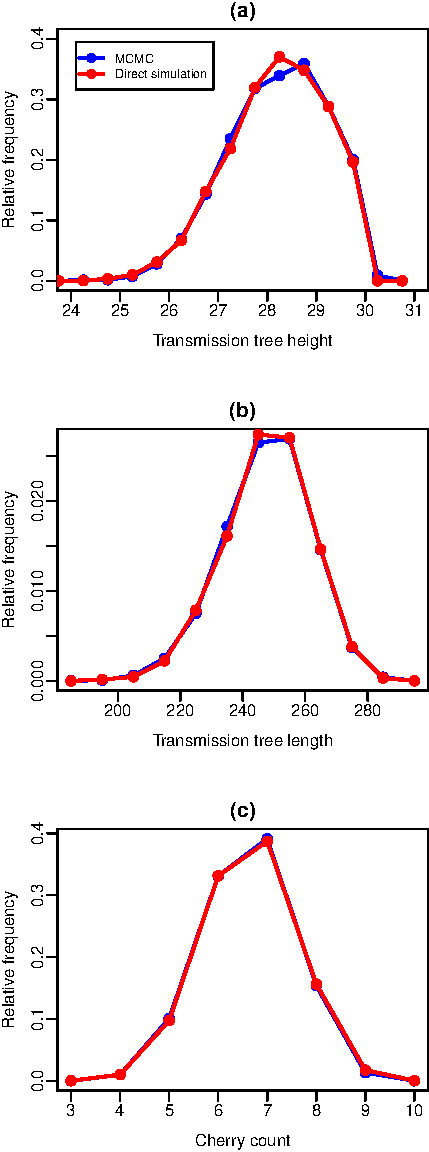
\includegraphics[width=0.6\textwidth]{detCoalFigure-crop.pdf}
    \end{center}
    \caption{Comparison between distributions of summary statistics of
      trees sampled using MCMC employing our implementation of the
      \emph{deterministic coalescent SIR model} likelihood and those
      calculated, and those of trees sampled using direct
      simulation. Summary statistics shown are (a) the age of the MRCA
      of the transmission tree, (b) the sum of all edge lengths in the
      tree and (c) the total number of two-leaf clades in the tree.}
    \label{fig:detCoalValidation}
\end{figure}

\begin{figure}
  \vspace{-3cm}

    \begin{center}
      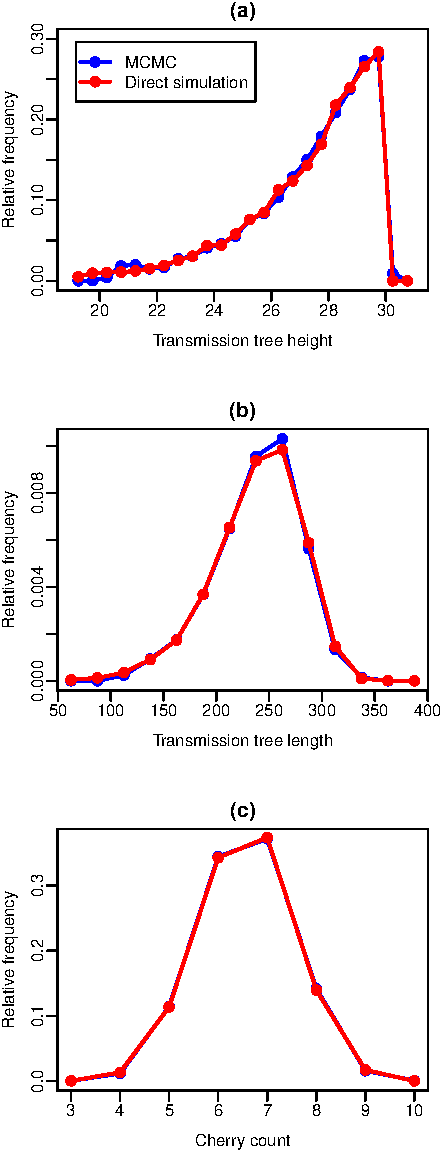
\includegraphics[width=0.6\textwidth]{stochCoalFigure-crop.pdf}
    \end{center}
    \caption{Comparison between distributions of summary statistics of
      trees sampled using MCMC employing our implementation of the
      \emph{stochastic coalescent SIR model} likelihood and those
      calculated, and those of trees sampled using direct
      simulation. Summary statistics shown are (a) the age of the MRCA
      of the transmission tree, (b) the sum of all edge lengths in the
      tree and (c) the total number of two-leaf clades in the tree.}
    \label{fig:stochCoalValidation}
\end{figure}

\begin{figure}
  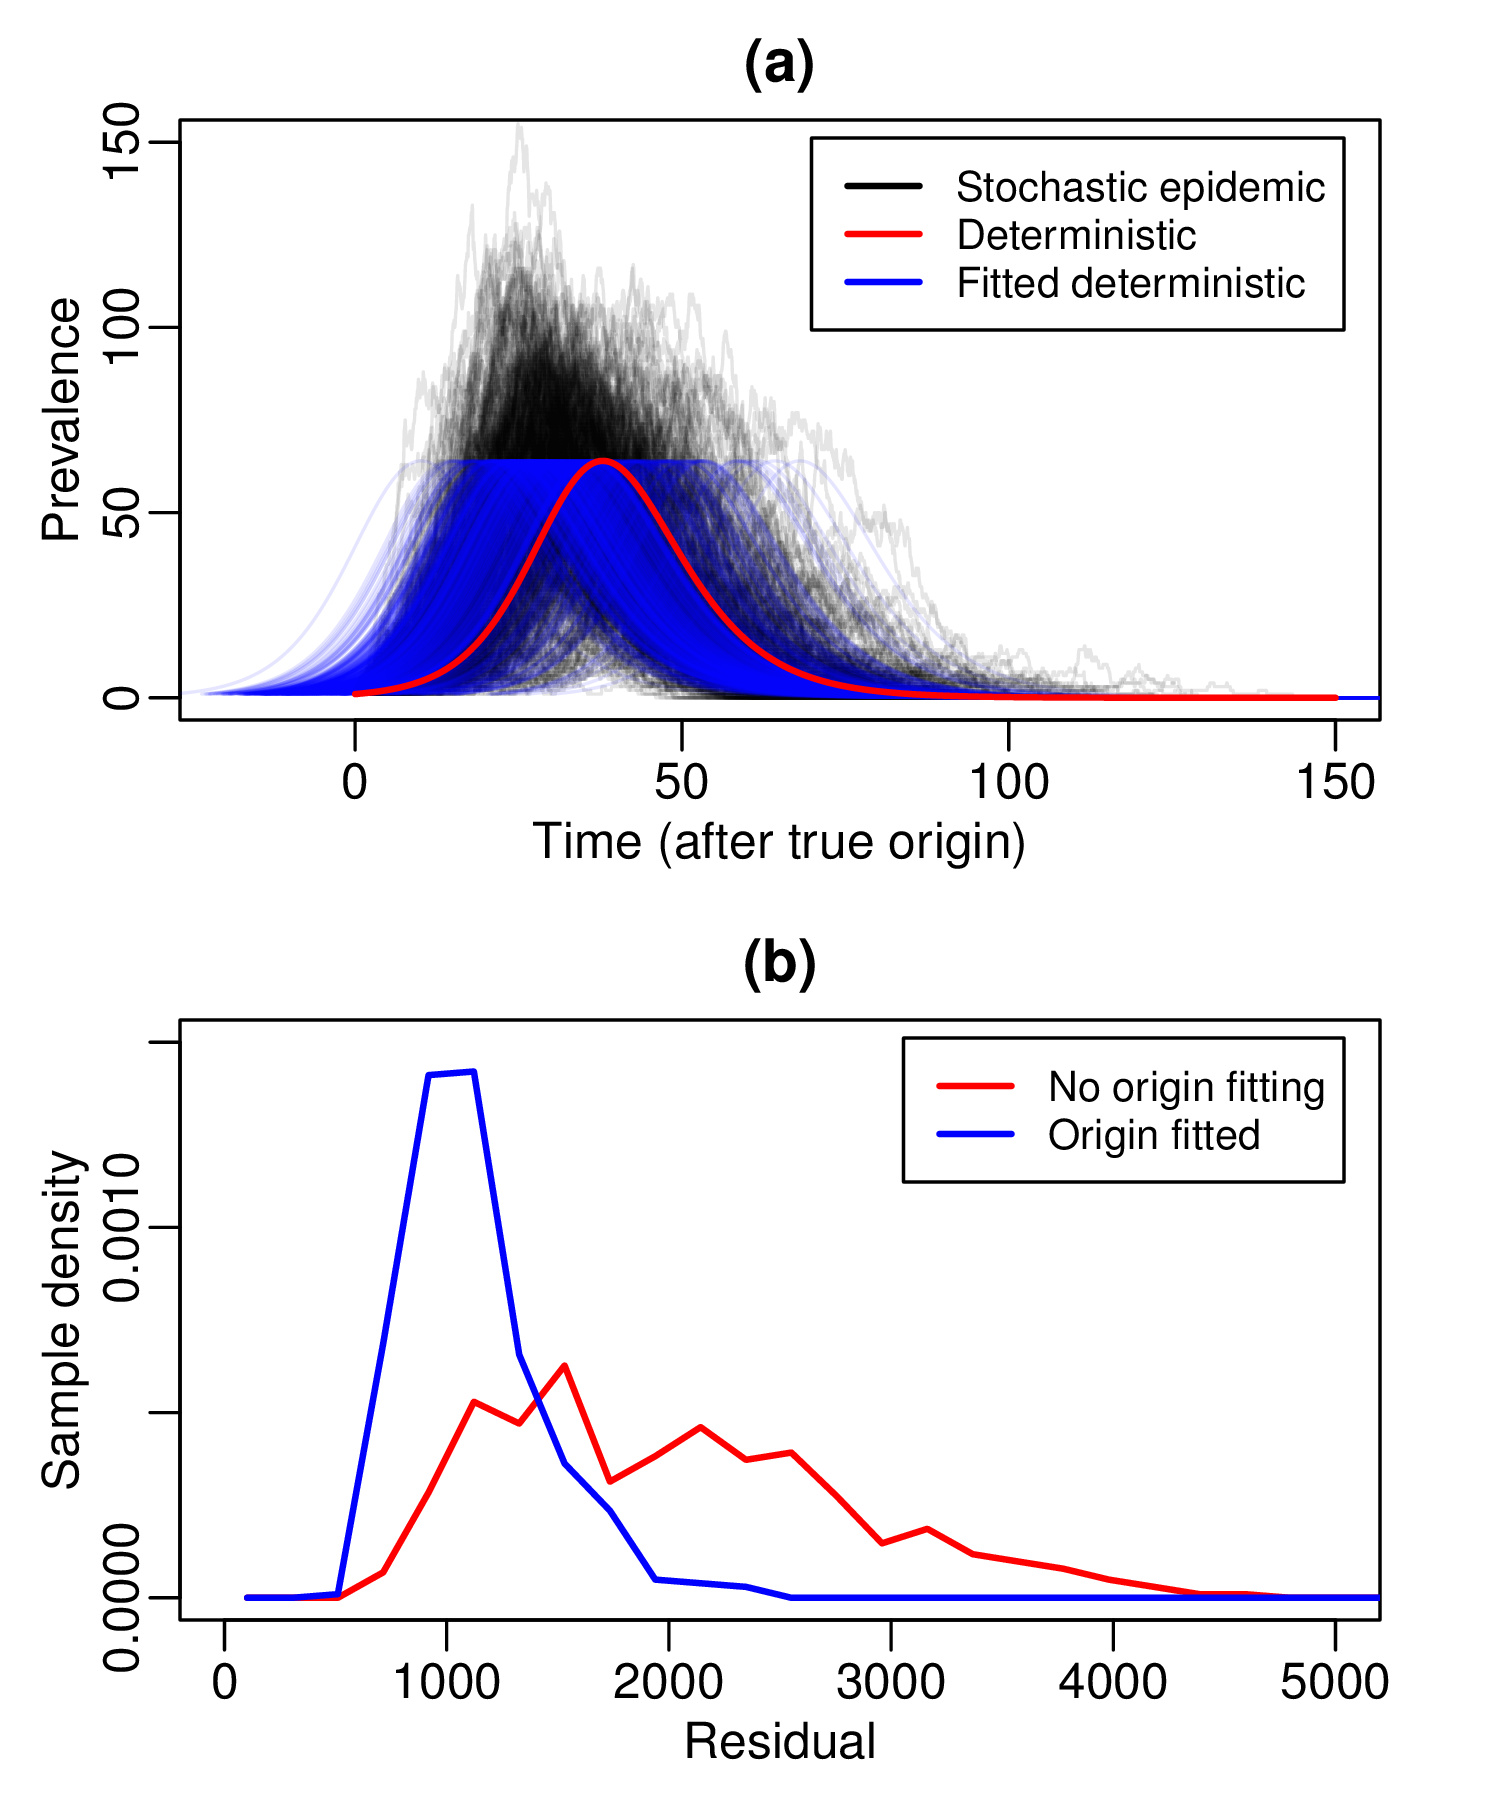
\includegraphics[width=\textwidth]{originFitFigure.jpg}
  \caption{(a) True stochastic SIR trajectories simulated jointly alongside phylogenies, with 
  the corresponding trajectories used by \deterCoalSIR{}.  Adjusting \deterCoalSIR{} 
  to fit the underlying stochastic trajectories causes major shifts to the origin $z_0$.  
  (b) Deterministic residuals with $z_0$ either fitted or not.}
  \label{fig:originFit}
\end{figure}

\begin{table}[!ht]
\begin{center}
\caption{\bf{Simulation Study Results for Stochastic Coalescent Trees}}
\begin{tabular}{|c|c|c|c|c|c|c|c|c|}
\hline
$\eta$ & Inference & Truth & Mean & Median & Error & Bias & Relative & 95\% HPD \\ 
&  &  &  &  &  &  &  HPD width & accuracy \\ 
	\hline
	\hline
$\mathcal{R}_0$ & Stoch.Coal.SIR & 2.50 & 2.81 & 2.64 & 0.11 & 0.08 & 0.95 & 100.00\% \\
& Deter.Coal.SIR & 2.50 & 2.73 & 2.65 & 0.14 & 0.06 & 0.85 & 96.00\% \\
   \hline
   \hline 
$\gamma$ & Stoch.Coal.SIR & 0.30 & 0.28 & 0.26 & 0.16 & -0.11 & 1.17 & 99.00\% \\
& Deter.Coal.SIR & 0.30 & 0.30 & 0.28 & 0.18 & -0.03 & 1.20 & 99.00\% \\
   \hline
   \hline
$S_{(0)}$ & Stoch.Coal.SIR & 999.00 & 1456.22 & 986.32 & 0.21 & 0.02 & 3.93 & 100.00\% \\
& Deter.Coal.SIR & 999.00 & 1719.88 & 1057.37 & 0.48 & 0.24 & 4.28 & 99.00\% \\
   \hline
   \hline
$z_{(0)}$ & Stoch.Coal.SIR & (varies) & 42.36 & 40.43 & 0.03 & 0.02 & 0.20 & 98.00\% \\
& Deter.Coal.SIR & (varies) & 41.25 & 39.77 & 0.03 & 0.01 & 0.07 & 64.00\% \\ 
   \hline
\end{tabular}
\end{center}
\label{table:simStochCoalTrees}
 \end{table}

\begin{table}[!ht]
\begin{center}
\caption{\bf{Simulation Study Results for Deterministic Coalescent Trees}}
\begin{tabular}{|c|c|c|c|c|c|c|c|c|}
\hline
$\eta$ & Inference & Truth & Mean & Median & Error & Bias & Relative & 95\% HPD \\ 
&  &  &  &  &  &  &  HPD width & accuracy \\ 
	\hline
	\hline
$\mathcal{R}_0$ & Stoch.Coal.SIR & 2.50 & 2.44 & 2.37 & 0.06 & -0.05 & 0.67 & 100.00\% \\
& Deter.Coal.SIR & 2.50 & 2.51 & 2.46 & 0.08 & -0.01 & 0.59 & 99.00\% \\
   \hline
   \hline 
$\gamma$ & Stoch.Coal.SIR & 0.30 & 0.33 & 0.31 & 0.07 & 0.05 & 1.00 & 100.00\% \\
& Deter.Coal.SIR & 0.30 & 0.32 & 0.30 & 0.10 & 0.02 & 0.79 & 100.00\% \\
   \hline
   \hline
$S_{(0)}$ & Stoch.Coal.SIR & 999.00 & 1586.15 & 1141.95 & 0.26 & 0.20 & 3.83 & 100.00\% \\
& Deter.Coal.SIR & 999.00 & 1426.32 & 1029.51 & 0.36 & 0.13 & 3.03 & 100.00\% \\
   \hline
   \hline
$z_{(0)}$ & Stoch.Coal.SIR & 44.12 & 45.52 & 44.74 & 0.02 & 0.01 & 0.19 & 93.00\% \\
& Deter.Coal.SIR & 44.12 & 44.34 & 44.11 & 0.02 & 1.93\mbox{\sc{e}-3} & 0.08 & 92.00\% \\
   \hline
\end{tabular}
\end{center}
\label{table:simDetCoalTrees}
 \end{table}

\begin{table}[!ht]
\small
\begin{center}
\caption{
\bf{Simulation Study Results:  $R_{0}=2.50$, $S_{0}=999$}}
\begin{tabular}{|c|c|c|c|c|c|c|c|c|}
\hline
$\eta$ & Inference & Truth & Mean & Median & Error & Bias & Relative & 95\% HPD \\ 
&  &  &  &  &  &  &  HPD width & accuracy \\ 
	\hline
	\hline
& Stoch.Coal.SIR & 2.50 & 2.84 & 2.68 & 0.12 & 0.09 & 0.98 & 100.00\% \\
$\mathcal{R}_0$ & Deter.Coal.SIR & 2.50 & 2.68 & 2.49 & 0.13 & 0.04 & 0.81 & 98.00\% \\
& \BDSIR{} & 2.50 & 2.73 & 2.67 & 0.12 & 0.08 & 0.55 & 94.00\%\\ 
   \hline
   \hline 
& Stoch.Coal.SIR & 0.30 & 0.27 & 0.25 & 0.19 & -0.13 & 1.14 & 99.00\% \\
$\gamma$ & Deter.Coal.SIR & 0.30 & 0.32 & 0.29 & 0.16 & 3.14\mbox{\sc{e}-3} & 1.27 & 99.00\% \\
& \BDSIR{} & 0.30 & 0.28 & 0.27 & 0.13 & -0.09 & 0.62 & 95.00\%\\ 
   \hline
   \hline
& Stoch.Coal.SIR & 999.00 & 1390.16 & 920.87 & 0.19 & -0.03 & 3.85 & 100.00\% \\
$S_{(0)}$ & Deter.Coal.SIR & 999.00 & 1807.18 & 1132.48 & 0.52 & 0.29 & 4.59 & 98.00\% \\
& \BDSIR{} & 999.00 & 1591.06 & 1141.88 & 0.39 & 0.24 & 3.42 & 99.00\% \\ 
   \hline
   \hline
& Stoch.Coal.SIR & (varies) & 41.81 & 40.35 & 0.03 & 0.01 & 0.20 & 99.00\% \\
$z_{(0)}$ & Deter.Coal.SIR & (varies) & 41.17 & 39.99 & 0.03 & 0.01 & 0.07 & 76.00\% \\
& \BDSIR{} & (varies) & 40.89 & 39.72 & 8.65\mbox{\sc{e}-4} & -5.13\mbox{\sc{e}-4} & 3.43\mbox{\sc{e}-3} & 97.00\% \\  
   \hline
\end{tabular}
\end{center}
{}
\label{table:sim}
\end{table}

\begin{table}[!ht]
\begin{center}
\caption{\bf{Simulation Study Results: $R_{0}=1.10$, $S_{0}=499$}}
\begin{tabular}{|c|c|c|c|c|c|c|c|c|}
\hline
$\eta$ & Inference & Truth & Mean & Median & Error & Bias & Relative & 95\% HPD \\ 
&  &  &  &  &  &  &  HPD width & accuracy \\ 
	\hline
	\hline
 & Stoch.Coal.SIR & 1.10 & 1.39 & 1.32 & 0.22 & 0.22 & 1.09 & 99.00\% \\
$\mathcal{R}_0$ & Deter.Coal.SIR & 1.10 & 1.68 & 1.44 & 0.46 & 0.46 & 0.59 & 25.00\% \\
 & BDSIR & 1.10 & 1.34 & 1.32 & 0.20 & 0.20 & 0.51 & 75.00\% \\
   \hline
   \hline 
 & Stoch.Coal.SIR & 0.25 & 0.17 & 0.15 & 0.37 & -0.36 & 1.11 & 84.00\% \\
$\gamma$ & Deter.Coal.SIR & 0.25 & 0.22 & 0.18 & 0.30 & -0.22 & 1.16 & 86.00\% \\
 & BDSIR & 0.25 & 0.28 & 0.26 & 0.12 & 0.09 & 0.92 & 100.00\% \\
   \hline
   \hline
 & Stoch.Coal.SIR & 499.00 & 608.16 & 397.92 & 0.24 & -0.18 & 3.38 & 100.00\% \\
$S_{(0)}$ & Deter.Coal.SIR & 499.00 & 553.38 & 337.10 & 0.42 & -0.26 & 3.08 & 92.00\% \\
 & BDSIR & 499.00 & 1471.05 & 1039.75 & 1.21 & 1.21 & 6.52 & 99.00\% \\
   \hline
   \hline
 & Stoch.Coal.SIR & (varies) & 91.60 & 84.55 & 0.06 & 0.02 & 0.60 & 97.00\% \\
$z_{(0)}$ & Deter.Coal.SIR & (varies) & 112.79 & 90.37 & 0.26 & 0.26 & 0.94 & 85.00\% \\
 & BDSIR & (varies) & 82.98 & 80.93 & 0.02 & -0.01 & 0.08 & 88.00\% \\
   \hline
\end{tabular}
\end{center}
\label{table:simLowerS0}
 \end{table}

 \begin{table}[!ht]
\begin{center}
\caption{
\bf{Simulation Study Results: Broader priors}}
\label{table:simLowerS0broadPriors}
\end{center}
\vspace{-0.4cm}
\hspace{-2cm}\begin{tabular}{|c|c|c|c|c|c|c|c|c|c|}
\hline
%$\eta$ & Inference & UpDown & Truth & Mean & Median & Error & Bias & Relative & 95\% HPD \\ 
%&  & Operator? &  &  &  &  &  & HPD width & accuracy \\ 
$\eta$ & Inference & St. Dev. & Truth & Mean & Median & Error & Bias & Relative & 95\% HPD \\ 
&  &  &  &  &  &  &  & HPD width & accuracy \\ 
	\hline
	\hline
$\mathcal{R}_0$ & Deter.Coal.SIR & 2 & 1.50 & 2.06 & 1.75 & 0.40 & 0.35 & 0.86 & 79.00\% \\
$\mathcal{R}_0$ & Deter.Coal.SIR & 1 & 1.50 & 1.80 & 1.49 & 0.24 & 0.15 & 0.52 & 85.00\% \\
%$\mathcal{R}_0$ & Deter.Coal.SIR & Yes & 1.50 & 2.06 & 1.76 & 0.40 & 0.35 & 0.87 & 80.00\% \\
$\mathcal{R}_0$ & Deter.Coal.SIR & 2 & 2.50 & 3.31 & 2.85 & 0.34 & 0.24 & 1.43 & 95.00\% \\
$\mathcal{R}_0$ & Deter.Coal.SIR & 1 & 2.50 & 2.68 & 2.49 & 0.13 & 0.04 & 0.80 & 99.00\% \\
%$\mathcal{R}_0$ & Deter.Coal.SIR & Yes & 2.50 & 3.32 & 2.86 & 0.34 & 0.25 & 1.42 & 93.00\% \\
   \hline
   \hline 
$\gamma$ & Deter.Coal.SIR & 2 & 0.30 & 0.31 & 0.23 & 0.37 & -0.12 & 1.59 & 96.00\% \\
$\gamma$ & Deter.Coal.SIR & 1 &0.30 & 0.26 & 0.23 & 0.27 & -0.22 & 1.15 & 89.00\% \\
%$\gamma$ & Deter.Coal.SIR & Yes & 0.30 & 0.30 & 0.23 & 0.38 & -0.12 & 1.65 & 95.00\% \\
$\gamma$ & Deter.Coal.SIR & 2 & 0.30 & 0.31 & 0.25 & 0.33 & -0.09 & 1.59 & 95.00\% \\
$\gamma$ & Deter.Coal.SIR & 1 &0.30 & 0.32 & 0.29 & 0.16 & 3.14\mbox{\sc{e}-3} & 1.27 & 99.00\% \\
%$\gamma$ & Deter.Coal.SIR & Yes & 0.30 & 0.31 & 0.25 & 0.32 & -0.10 & 1.65 & 94.00\% \\
   \hline
   \hline
$S_{(0)}$ & Deter.Coal.SIR & 2 & 499.00 & 2040.5 & 249.27 & 1.40 & 0.49 & 7.75 & 85.00\% \\
$S_{(0)}$ & Deter.Coal.SIR & 1 & 499.00 & 561.72 & 361.36 & 0.44 & -0.26 & 3.36 & 91.00\% \\
%$S_{(0)}$ & Deter.Coal.SIR & Yes & 499.00 & 2066.28 & 252.13 & 1.41 & 0.50 & 8.04 & 84.00\% \\
$S_{(0)}$ & Deter.Coal.SIR & 2 & 999.00 & 3028.13 & 716.46 & 1.05 & 0.33 & 6.60 & 94.00\% \\
$S_{(0)}$ & Deter.Coal.SIR & 1 & 499.00 & 553.38 & 337.10 & 0.42 & -0.26 & 3.08 & 92.00\% \\
%$S_{(0)}$ & Deter.Coal.SIR & Yes & 999.00 & 3063.46 & 709.24 & 1.04 & 0.32 & 6.56 & 92.00\% \\
   \hline
   \hline
$z_{(0)}$ & Deter.Coal.SIR & 2 & (varies) & 65.10 & 62.01 & 0.04 & 0.03 & 0.25 & 86.00\% \\
$z_{(0)}$ & Deter.Coal.SIR & 1 & (varies) & 91.03 & 72.51 & 0.39 & 0.38 & 0.42 & 88.00\% \\
%$z_{(0)}$ & Deter.Coal.SIR & Yes & (varies) & 64.95 & 61.98 & 0.04 & 0.03 & 0.24 & 87.00\% \\
$z_{(0)}$ & Deter.Coal.SIR & 2 & (varies) & 40.97 & 39.85 & 0.03 & -6.78\mbox{\sc{e}-4} & 0.08 & 81.00\% \\
$z_{(0)}$ & Deter.Coal.SIR & 1 & (varies) & 112.79 & 90.37 & 0.26 & 0.26 & 0.94 & 85.00\% \\
%$z_{(0)}$ & Deter.Coal.SIR & Yes & (varies) & 40.97 & 39.84 & 0.03 & -7.64\mbox{\sc{e}-4} & 0.08 & 82.00\% \\
   \hline
\end{tabular}
\end{table}

%\begin{table}[!ht]
%\small
%\begin{center}
%\caption{
%\bf{Simulation Study Results:  100-tip trees}}
%\begin{tabular}{|c|c|c|c|c|c|c|c|c|}
%\hline
%$\eta$ & Inference & Truth & Mean & Median & Error & Bias & Relative & 95\% HPD \\ 
%&  &  &  &  &  &  &  HPD width & accuracy \\ 
%	\hline
%	\hline
%$\mathcal{R}_0$ & Deter.Coal.SIR & 2.50 & 3.15 & 2.83 & 0.18 & 0.12 & 1.70 & 100.00\% \\
%$\mathcal{R}_0$ & Deter.Coal.SIR & 1.50 & 1.89 & 1.70 & 0.21 & 0.19 & 0.84 & 96.00\% \\
%$\mathcal{R}_0$ & Deter.Coal.SIR & 1.10 & 1.81 & 1.50 & 0.58 & 0.58 & 0.73 & 17.00\% \\
%   \hline
%   \hline 
%$\gamma$ & Deter.Coal.SIR & 0.30 & 0.29 & 0.26 & 0.24 & -0.12 & 1.77 & 100.00\% \\
%$\gamma$ & Deter.Coal.SIR & 0.30 & 0.25 & 0.22 & 0.30 & -0.23 & 1.32 & 93.00\% \\
%$\gamma$ & Deter.Coal.SIR & 0.25 & 0.26 & 0.23 & 0.22 & -0.06 & 1.39 & 93.00\% \\
%   \hline
%   \hline
%$S_{(0)}$ & Deter.Coal.SIR & 999.00 & 2254.25 & 1261.90 & 0.60 & 0.49 & 5.80 & 100.00\% \\
%$S_{(0)}$ & Deter.Coal.SIR & 499.00 & 773.85 & 460.43 & 0.36 & 0.03 & 4.36 & 99.00\% \\
%$S_{(0)}$ & Deter.Coal.SIR & 499.00 & 577.30 & 363.86 & 0.45 & -0.23 & 3.36 & 91.00\% \\
%   \hline
%   \hline
%$z_{(0)}$ & Deter.Coal.SIR & (varies) & 20.09 & 19.77 &  &  &  & \% \\
%$z_{(0)}$ & Deter.Coal.SIR & (varies) & 45.27 & 38.02 &  &  &  & \% \\
%$z_{(0)}$ & Deter.Coal.SIR & (varies) & 91.67 &  &  &  &  & \% \\
%   \hline
%\end{tabular}
%\end{center}
%{}
%\label{table:sim}
%\end{table}

% Flush all outstanding floats
\clearpage

\bibliography{../volzSIR}
\bibliographystyle{../genetics}
\end{document}